%% ============================================================
%%  Treehouse Ghana Instagram Intelligence Report
%%  GENERATED by src/generate_combined_report.js from config + CSVs.
%%  Do not edit by hand; edit config/client.config.json and re-run.
%%  Odwira and Whitehall — Bernard Ashiley — 2026-05-31
%% ============================================================
\documentclass[11pt,a4paper]{report}
\usepackage[a4paper, top=2.5cm, bottom=2.5cm, left=2.8cm, right=2.8cm]{geometry}
\usepackage[T1]{fontenc}\usepackage[utf8]{inputenc}\usepackage{lmodern}\usepackage{microtype}
\usepackage{xcolor}\usepackage{booktabs}\usepackage{longtable}\usepackage{array}\usepackage{tabularx}
\usepackage{parskip}\usepackage{titlesec}\usepackage{fancyhdr}\usepackage{pgfplots}\usepackage{tikz}
\usepackage{hyperref}\usepackage{enumitem}\usepackage{caption}\usepackage{mdframed}\usepackage{amsmath}
\pgfplotsset{compat=1.18}
\definecolor{tggreen}{HTML}{1B3A2D}\definecolor{tgmid}{HTML}{2D6A4F}
\definecolor{tglight}{HTML}{D8F3DC}\definecolor{tggold}{HTML}{C9A84C}
\definecolor{tgblue}{HTML}{2E86AB}\definecolor{tgpurple}{HTML}{7B2D8B}
\definecolor{tggrey}{HTML}{4B5563}\definecolor{tglightgrey}{HTML}{F3F4F6}\definecolor{tgrule}{HTML}{D1D5DB}
\hypersetup{colorlinks=true,linkcolor=tggreen,urlcolor=tgblue,pdfauthor={Bernard Ashiley -- Odwira and Whitehall},pdftitle={Treehouse Ghana Instagram Intelligence Report}}
\titleformat{\chapter}[display]{\normalfont\Large\bfseries\color{tggreen}}{\chaptername\ \thechapter}{10pt}{\Huge}
\titleformat{\section}{\normalfont\large\bfseries\color{tggreen}}{}{0em}{}[\color{tgrule}\titlerule]
\titleformat{\subsection}{\normalfont\normalsize\bfseries\color{tgmid}}{}{0em}{}
\pagestyle{fancy}\fancyhf{}
\fancyhead[L]{\small\color{tggrey}\textit{Treehouse Ghana Instagram Intelligence Report}}
\fancyhead[R]{\small\color{tggrey}\textit{Odwira and Whitehall --- Confidential}}
\fancyfoot[C]{\small\color{tggrey}\thepage}
\renewcommand{\headrulewidth}{0.4pt}\renewcommand{\headrule}{\color{tgrule}\hrule width\headwidth height\headrulewidth}
\newmdenv[linecolor=tggreen,backgroundcolor=tglight,linewidth=1pt,roundcorner=4pt,innerleftmargin=12pt,innerrightmargin=12pt,innertopmargin=10pt,innerbottommargin=10pt]{callout}
\newmdenv[linecolor=tggold,backgroundcolor=tglightgrey,linewidth=1pt,roundcorner=4pt,innerleftmargin=12pt,innerrightmargin=12pt,innertopmargin=10pt,innerbottommargin=10pt]{note}
\newcolumntype{L}[1]{>{\raggedright\arraybackslash}p{#1}}
\newcolumntype{R}[1]{>{\raggedleft\arraybackslash}p{#1}}
\newcolumntype{C}[1]{>{\centering\arraybackslash}p{#1}}
\captionsetup{font=small, labelfont={bf,color=tggreen}, labelsep=period, skip=4pt}

\begin{document}

%% COVER
\begin{titlepage}\pagecolor{tggreen}\color{white}\vspace*{3cm}\begin{center}
{\fontsize{11}{13}\selectfont\textit{Odwira and Whitehall}}\\[6pt]
{\color{tggold}\rule{6cm}{1pt}}\\[28pt]
{\fontsize{34}{40}\selectfont\bfseries Treehouse Ghana}\\[10pt]
{\fontsize{18}{24}\selectfont Instagram Intelligence Report}\\[18pt]
{\color{tggold}\rule{10cm}{0.6pt}}\\[22pt]
{\fontsize{12}{16}\selectfont Public engagement, audience intent, and content strategy analysis\\[4pt]
Prepared from public Instagram data for Treehouse Ghana (\texttt{@treehousegh})}\\[40pt]
{\fontsize{11}{14}\selectfont \textbf{Prepared by:} Bernard Ashiley\\[4pt]\textbf{Organisation:} Odwira and Whitehall\\[4pt]\textbf{Date:} 2026-05-31\\[4pt]\textbf{Classification:} Confidential}
\end{center}\vfill\begin{center}{\small\color{white!70!tggreen}This document integrates a performance overview, a detailed engagement analysis, and a full advanced statistical and predictive analysis including Monte Carlo simulation. It is exploratory and fully reproducible; see the Statistical Scope section.}\end{center}\end{titlepage}
\nopagecolor
\tableofcontents
\newpage

\part{Performance Overview}
\chapter{At a Glance}
All metrics are derived entirely from public data. Private account analytics (reach, impressions, saves, shares, profile visits, link clicks) are excluded and remain visible only within the native Instagram Insights dashboard.

\vspace{10pt}
\begin{callout}
\begin{tabularx}{\linewidth}{@{}L{4.2cm} X@{}}
  \textbf{Followers}            & 27,386 at time of collection \\[4pt]
  \textbf{Posts analysed}       & 135 owned feed posts and 84 short videos (reels) \\[4pt]
  \textbf{Top content category} & Cocktails and Drinks (average engagement score: 290) \\[4pt]
  \textbf{Best day to post}     & Monday (average engagement score: 199) \\[4pt]
  \textbf{Format signal}        & Short videos show higher interaction; advantage is directional (see Reels vs Posts) \\
\end{tabularx}
\end{callout}

\section{Data Coverage}
\begin{table}[htbp]
\centering
\caption{Summary of data collected for analysis}
\begin{tabular}{@{}L{7cm} R{4cm}@{}}
\toprule
\textbf{Area} & \textbf{Count} \\
\midrule
Owned feed posts analysed & 135 \\
Reels analysed & 84 \\
Third-party mentions analysed & 21 \\
Comments analysed & 106 \\
Followers at collection time & 27,386 \\
\bottomrule
\end{tabular}
\end{table}

Profile biography: \textit{Al fresco dining in the heart of Accra. Open daily from noon to 11pm.}

\begin{note}
\textbf{Data limitation.} This analysis covers public Instagram data only. It does not include private account analytics such as reach, impressions, saves, shares, profile visits, link clicks, story taps, ad spend, or completed bookings. All conclusions are directional rather than absolute. Combine these findings with Treehouse Ghana's native Instagram analytics, reservation data, and campaign context.
\end{note}


\chapter{Content Performance}
\section{Engagement Score Methodology}
The engagement score used throughout is:
\begin{equation*}\text{Engagement Score} = \text{Likes} + (\text{Comments}\times 5) + \left(\tfrac{\text{Views or Plays}}{100}\right)\end{equation*}
It is a consistent, reproducible index for comparing posts on partial public metrics, not a replacement for native analytics. Comments are weighted at five times a like because they require active intent.

\begin{note}
\textbf{Important caveat on the views term.} The views/plays component is available almost exclusively for video. In this dataset, image posts frequently record zero views while reels do not. The composite score therefore structurally favours video, and any reels-versus-image comparison \emph{on the composite score} is partly a property of the formula. Comparisons that this affects are also reported on likes and comments alone (see Section~\ref{sec:reelsposts}).
\end{note}

\section{What Content Performs Best}
\begin{figure}[htbp]
\centering
\caption{Average engagement score by content pillar}
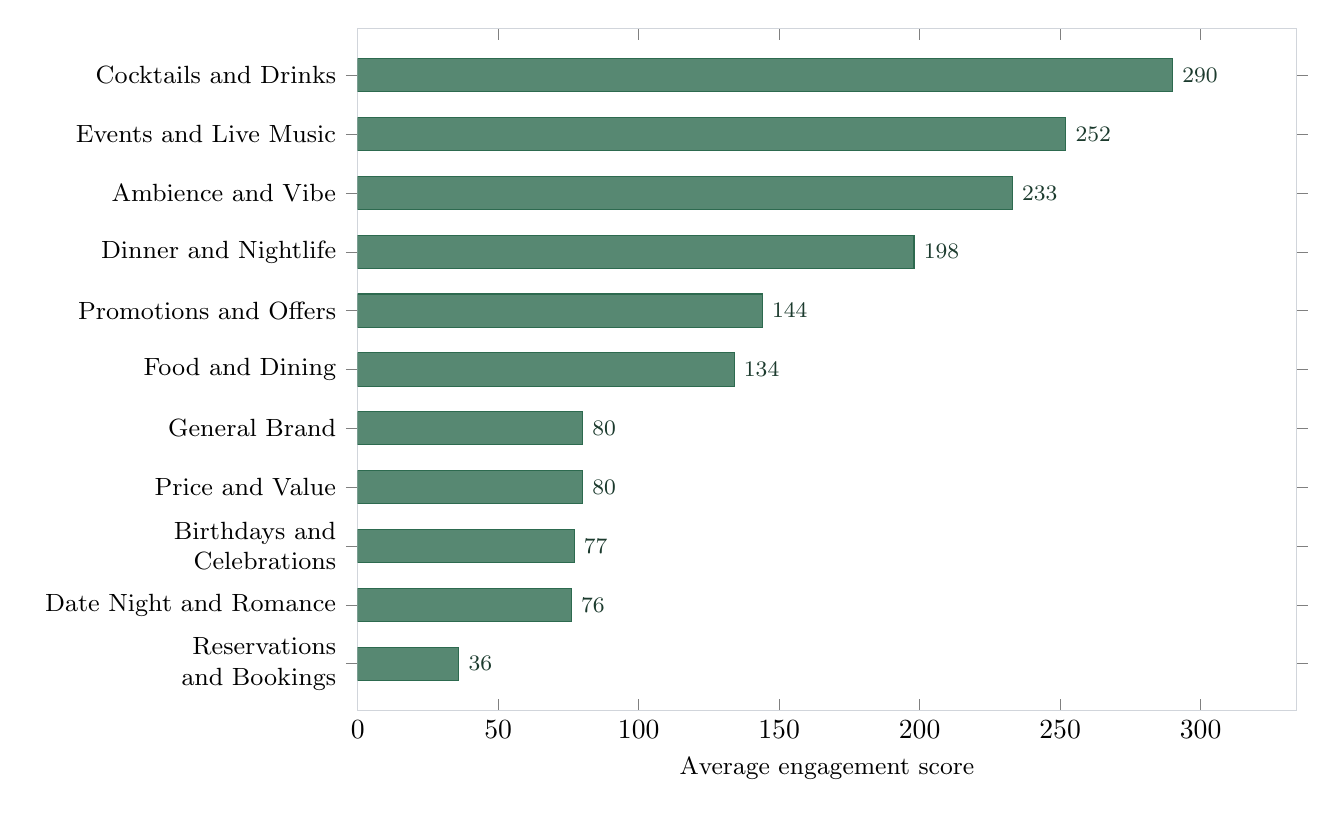
\begin{tikzpicture}
\begin{axis}[
  xbar, xmin=0, xmax=334,
  width=13.5cm, height=10.25cm, bar width=12pt,
  xlabel={\small Average engagement score},
  symbolic y coords={Reservations and Bookings,Date Night and Romance,Birthdays and Celebrations,Price and Value,General Brand,Food and Dining,Promotions and Offers,Dinner and Nightlife,Ambience and Vibe,Events and Live Music,Cocktails and Drinks}, ytick=data,
  y tick label style={font=\small, align=right, text width=3.8cm},
  scaled x ticks=false,
  xticklabel style={/pgf/number format/.cd,fixed,fixed zerofill=false,precision=0,1000 sep={,}},
  nodes near coords={\pgfmathprintnumber[fixed,precision=0,1000 sep={,}]{\pgfplotspointmeta}},
  nodes near coords align={horizontal},
  every node near coord/.style={font=\footnotesize, color=tggreen},
  enlarge y limits=0.08, axis line style={draw=tgrule},
]
\addplot[fill=tgmid!80, draw=tgmid] coordinates {(36,Reservations and Bookings)(76,Date Night and Romance)(77,Birthdays and Celebrations)(80,Price and Value)(80,General Brand)(134,Food and Dining)(144,Promotions and Offers)(198,Dinner and Nightlife)(233,Ambience and Vibe)(252,Events and Live Music)(290,Cocktails and Drinks)};
\end{axis}
\end{tikzpicture}
\end{figure}

\section{Full Content Pillar Breakdown}
\begin{longtable}{@{}L{4cm} R{1.6cm} R{2cm} R{2cm} R{2cm} R{2.2cm}@{}}
\caption{Content pillar performance summary} \\
\toprule
\textbf{Pillar} & \textbf{Posts} & \textbf{Avg Likes} & \textbf{Avg Cmts} & \textbf{Avg Views} & \textbf{Avg Score} \\
\midrule
\endfirsthead
\multicolumn{6}{c}{\tablename\ \thetable{} --- continued} \\
\toprule
\textbf{Pillar} & \textbf{Posts} & \textbf{Avg Likes} & \textbf{Avg Cmts} & \textbf{Avg Views} & \textbf{Avg Score} \\
\midrule
\endhead
\bottomrule
\endfoot
\bottomrule
\endlastfoot
Cocktails and Drinks & 11 & 132 & 2.91 & 14,304 & 289.59 \\
Events and Live Music & 8 & 121.75 & 2.38 & 11,830 & 251.93 \\
Ambience and Vibe & 15 & 123.07 & 14.2 & 3,869 & 232.75 \\
Dinner and Nightlife & 17 & 86.71 & 2.06 & 10,094 & 197.94 \\
Promotions and Offers & 2 & 72 & 1 & 6,681 & 143.81 \\
Food and Dining & 111 & 61.42 & 0.98 & 6,739 & 133.73 \\
General Brand & 33 & 57.15 & 2.79 & 927 & 80.36 \\
Price and Value & 2 & 54 & 1 & 2,084 & 79.84 \\
Birthdays and Celebrations & 6 & 31.67 & 0.33 & 4,340 & 76.73 \\
Date Night and Romance & 12 & 49.25 & 0.42 & 2,474 & 76.07 \\
Reservations and Bookings & 2 & 19 & 0 & 1,654 & 35.54 \\
\end{longtable}

\begin{note}
\textbf{How to read these rankings.} Categories are ordered by average engagement score, but several rest on very few posts. Categories with fewer than ten posts have unstable averages and wide confidence intervals (Part~II); treat them as hypotheses worth testing with more content, not settled rankings.
\end{note}

\chapter{Short Videos versus Feed Posts}
\section{Comparative Performance}\label{sec:reelsposts}
This account has \textbf{134 feed posts and 16 reels} in the analysed window. The engagement score embeds a views term available to video but not to many image posts (49\% of feed posts here record zero views), so the comparison is shown three ways: on the composite score, and on likes-and-comments and likes alone, which remove that mechanical advantage.

\begin{table}[htbp]
\centering
\caption{Reels versus posts under three metrics (deduplicated data)}
\begin{tabular}{@{}L{6cm} R{2cm} R{2cm} R{2cm}@{}}
\toprule
\textbf{Metric} & \textbf{Reel mean} & \textbf{Post mean} & \textbf{MWU p-value} \\
\midrule
Engagement score (includes views) & 248 & 112 & 0.057 \\
Likes + comments only (no views) & 121 & 71 & 0.179 \\
Likes only & 103 & 62 & 0.557 \\
\bottomrule
\end{tabular}
\end{table}

\begin{callout}
\textbf{Honest reading.} Short videos lead on the composite score, but much of that gap is the mechanical views term; on likes and comments the difference is not statistically reliable at this sample size. Treat reels as a reach and discovery investment and confirm with native reach data.
\end{callout}

\chapter{Timing Analysis}
\section{Best Days to Post}
\begin{figure}[htbp]
\centering
\caption{Average engagement score by posting day}
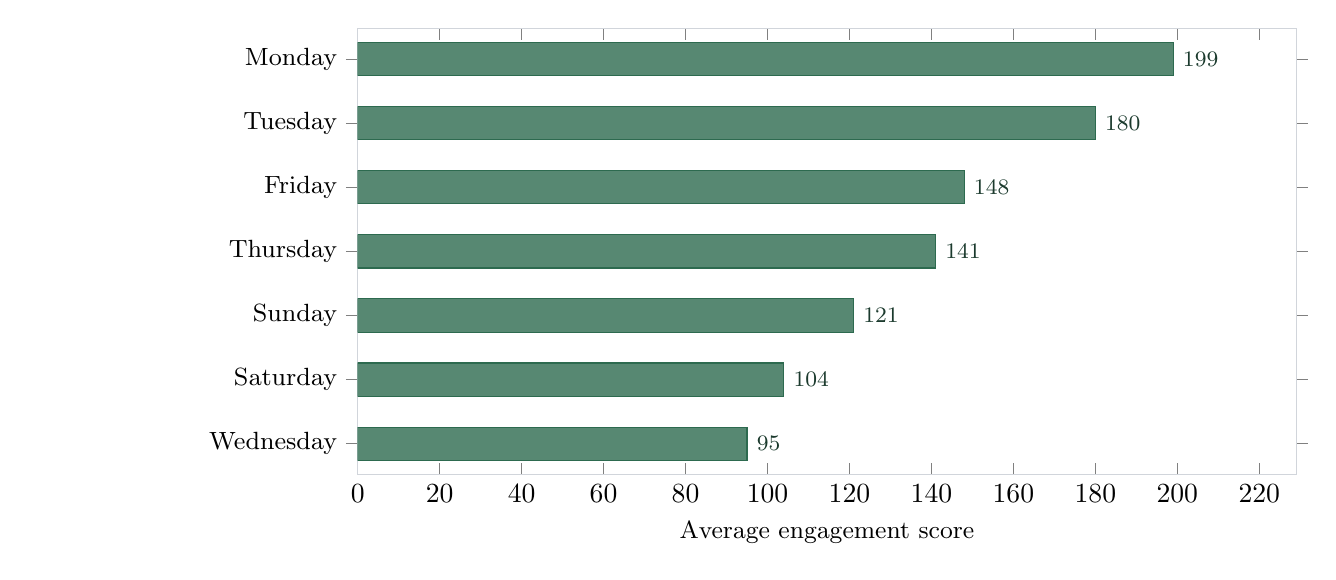
\begin{tikzpicture}
\begin{axis}[
  xbar, xmin=0, xmax=229,
  width=13.5cm, height=7.25cm, bar width=12pt,
  xlabel={\small Average engagement score},
  symbolic y coords={Wednesday,Saturday,Sunday,Thursday,Friday,Tuesday,Monday}, ytick=data,
  y tick label style={font=\small, align=right, text width=3.8cm},
  scaled x ticks=false,
  xticklabel style={/pgf/number format/.cd,fixed,fixed zerofill=false,precision=0,1000 sep={,}},
  nodes near coords={\pgfmathprintnumber[fixed,precision=0,1000 sep={,}]{\pgfplotspointmeta}},
  nodes near coords align={horizontal},
  every node near coord/.style={font=\footnotesize, color=tggreen},
  enlarge y limits=0.08, axis line style={draw=tgrule},
]
\addplot[fill=tgmid!80, draw=tgmid] coordinates {(95,Wednesday)(104,Saturday)(121,Sunday)(141,Thursday)(148,Friday)(180,Tuesday)(199,Monday)};
\end{axis}
\end{tikzpicture}
\end{figure}

\begin{table}[htbp]
\centering
\caption{Timing analysis by day of week}
\begin{tabular}{@{}L{2.8cm} R{2cm} R{2.2cm} R{2cm} R{2.2cm}@{}}
\toprule
\textbf{Day} & \textbf{Posts} & \textbf{Avg Score} & \textbf{Avg Likes} & \textbf{Avg Cmts} \\
\midrule
Monday & 20 & 198.86 & 99.15 & 1.9 \\
Tuesday & 43 & 179.97 & 75.14 & 3.33 \\
Friday & 47 & 147.64 & 77.53 & 1.55 \\
Thursday & 38 & 141.39 & 62.39 & 0.74 \\
Sunday & 17 & 120.65 & 79.94 & 3.41 \\
Saturday & 27 & 104.15 & 53.44 & 5.56 \\
Wednesday & 27 & 94.56 & 55.19 & 0.78 \\
\bottomrule
\end{tabular}
\end{table}

\section{Timing by Hour (UTC)}
\begin{longtable}{@{}R{2.5cm} R{2cm} R{2.8cm} R{2cm} R{2.2cm}@{}}
\caption{Average engagement by publication hour (UTC)} \\
\toprule
\textbf{Hour UTC} & \textbf{Posts} & \textbf{Avg Score} & \textbf{Avg Likes} & \textbf{Avg Cmts} \\
\midrule
\endfirsthead
\multicolumn{5}{c}{\tablename\ \thetable{} --- continued} \\
\toprule
\textbf{Hour UTC} & \textbf{Posts} & \textbf{Avg Score} & \textbf{Avg Likes} & \textbf{Avg Cmts} \\
\midrule
\endhead
\bottomrule
\endfoot
\bottomrule
\endlastfoot
Unknown & 3 & 44.85 & 15.67 & 2 \\
2 & 1 & 97 & 67 & 6 \\
3 & 6 & 62.78 & 27.67 & 5.33 \\
4 & 2 & 31.5 & 29 & 0.5 \\
7 & 2 & 80.73 & 64 & 1 \\
8 & 2 & 61.58 & -1 & 0 \\
9 & 8 & 61.96 & 26.5 & 0.75 \\
10 & 3 & 79.84 & 13.67 & 4.33 \\
11 & 5 & 765.42 & 408.6 & 2.8 \\
12 & 69 & 58.93 & 35.87 & 0.38 \\
13 & 21 & 232.02 & 82.48 & 2.71 \\
14 & 8 & 232.27 & 113 & 4.13 \\
15 & 34 & 161.25 & 76.59 & 0.79 \\
16 & 21 & 245.74 & 118.95 & 5.81 \\
17 & 6 & 69.61 & 21.17 & 2.67 \\
18 & 9 & 249.87 & 158.44 & 7 \\
19 & 5 & 32.82 & 7 & 0.2 \\
20 & 6 & 65.08 & 45 & 1 \\
21 & 6 & 208.15 & 115.33 & 13.33 \\
22 & 2 & 8.06 & -1 & 0 \\
\end{longtable}

\chapter{Audience Comment Intelligence}
The comment review uses anonymised text only; usernames are excluded from all outputs.

\begin{figure}[htbp]
\centering
\caption{Comment intent categories}
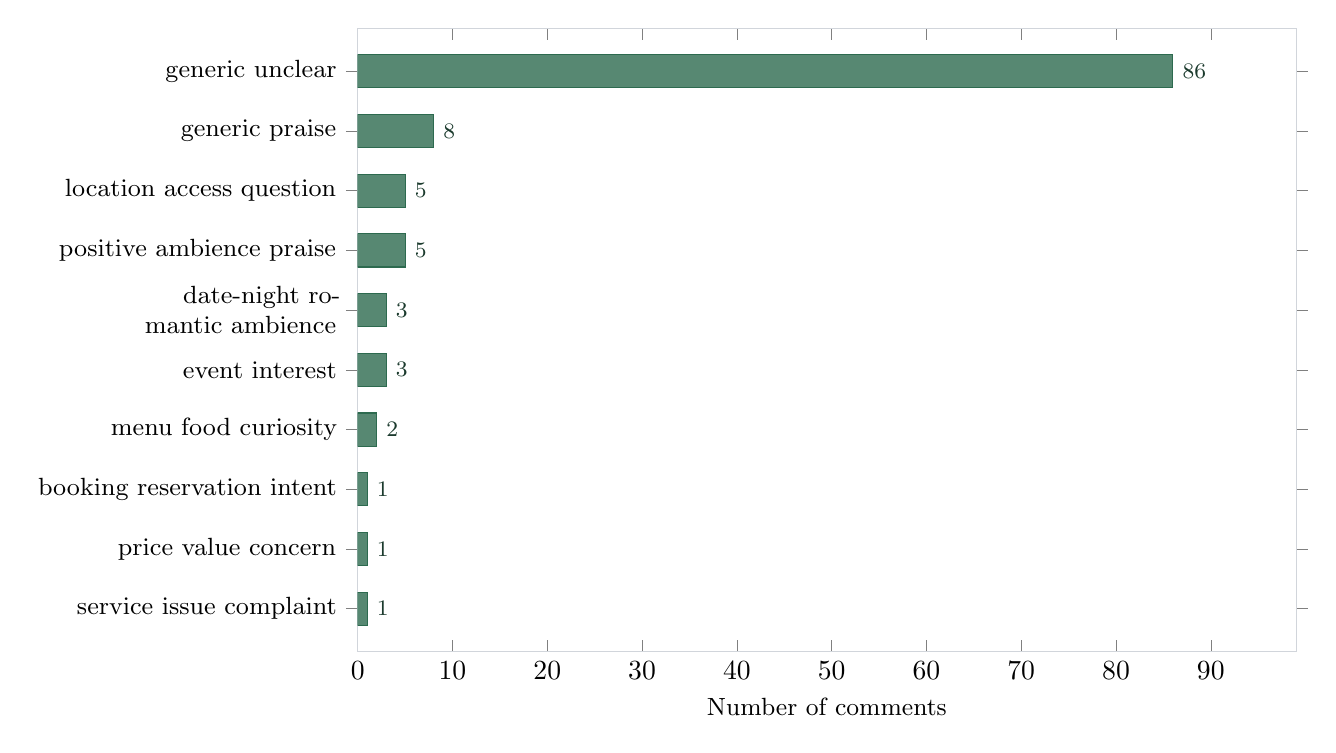
\begin{tikzpicture}
\begin{axis}[
  xbar, xmin=0, xmax=99,
  width=13.5cm, height=9.5cm, bar width=12pt,
  xlabel={\small Number of comments},
  symbolic y coords={service issue complaint,price value concern,booking reservation intent,menu food curiosity,event interest,date-night romantic ambience,positive ambience praise,location access question,generic praise,generic unclear}, ytick=data,
  y tick label style={font=\small, align=right, text width=3.8cm},
  scaled x ticks=false,
  xticklabel style={/pgf/number format/.cd,fixed,fixed zerofill=false,precision=0,1000 sep={,}},
  nodes near coords={\pgfmathprintnumber[fixed,precision=0,1000 sep={,}]{\pgfplotspointmeta}},
  nodes near coords align={horizontal},
  every node near coord/.style={font=\footnotesize, color=tggreen},
  enlarge y limits=0.08, axis line style={draw=tgrule},
]
\addplot[fill=tgmid!80, draw=tgmid] coordinates {(1,service issue complaint)(1,price value concern)(1,booking reservation intent)(2,menu food curiosity)(3,event interest)(3,date-night romantic ambience)(5,positive ambience praise)(5,location access question)(8,generic praise)(86,generic unclear)};
\end{axis}
\end{tikzpicture}
\end{figure}

\begin{longtable}{@{}L{4cm} R{1.4cm} R{1.4cm} L{7.5cm}@{}}
\caption{Full comment intent classification with commercial opportunities} \\
\toprule
\textbf{Intent} & \textbf{Count} & \textbf{Share} & \textbf{Commercial Opportunity} \\
\midrule
\endfirsthead
\multicolumn{4}{c}{\tablename\ \thetable{} --- continued} \\
\toprule
\textbf{Intent} & \textbf{Count} & \textbf{Share} & \textbf{Commercial Opportunity} \\
\midrule
\endhead
\bottomrule
\endfoot
\bottomrule
\endlastfoot
generic/unclear & 86 & 81.1\% & Useful brand warmth, but convert with clearer next steps. \\
generic praise & 8 & 7.5\% & Useful brand warmth, but convert with clearer next steps. \\
positive ambience praise & 5 & 4.7\% & Use ambience comments as proof for venue positioning. \\
location/access question & 5 & 4.7\% & Pin address, parking, map, and arrival guidance in captions and highlights. \\
event interest & 3 & 2.8\% & Create event posts with dates, times, line-up, and reservation CTA. \\
date-night/romantic ambience & 3 & 2.8\% & Package ambience-led content around date-night reservations. \\
menu/food curiosity & 2 & 1.9\% & Use captions and carousel slides to answer menu questions before users ask. \\
service issue/complaint & 1 & 0.9\% & Track and resolve operational issues privately; avoid letting concerns sit unanswered. \\
price/value concern & 1 & 0.9\% & Add menu ranges, bundles, or occasion packages where commercially appropriate. \\
booking/reservation intent & 1 & 0.9\% & Reply quickly with booking link or WhatsApp prompt and save FAQs to highlights. \\
\end{longtable}

\chapter{Caption and Hashtag Analysis}
\begin{table}[htbp]
\centering
\caption{Caption and hashtag summary statistics}
\begin{tabular}{@{}L{7cm} R{4cm}@{}}
\toprule
\textbf{Metric} & \textbf{Value} \\
\midrule
Average caption length & 192.7 characters \\
Median caption length & 151 characters \\
Average hashtags per post/reel & 3.69 \\
Average mentions per post/reel & 1.24 \\
\bottomrule
\end{tabular}
\end{table}

\section{Most Frequent Hashtags}
\begin{table}[htbp]
\centering
\caption{Top 15 hashtags by frequency of use}
\begin{tabular}{@{}L{5cm} R{3cm}@{}}
\toprule
\textbf{Hashtag} & \textbf{Uses} \\
\midrule
\#treehouserestaurant & 111 \\
\#reels & 54 \\
\#dinner & 47 \\
\#goodfood & 42 \\
\#explore & 35 \\
\#lunch & 21 \\
\#soulmusic & 19 \\
\#food & 19 \\
\#afroson1cx & 14 \\
\#livemusic & 12 \\
\#treehouse & 11 \\
\#afx2026 & 10 \\
\#foodinsta & 10 \\
\#dinnertime & 10 \\
\#soulfriday & 10 \\
\bottomrule
\end{tabular}
\end{table}

\part{Advanced Statistical and Predictive Analysis}

\chapter{Methodology and Data Quality}
All computation runs in a reproducible Node.js pipeline. Monte Carlo simulations use a fixed seed (20260530) and 10,000 iterations; an independent analyst re-running the code obtains bit-identical results. After removing duplicate posts that appear in both the posts and reels scrapes, the working dataset comprises \textbf{150 unique posts and reels} (107 published by the account, the remainder features and mentions).

\chapter{Exploratory Data Analysis}
\begin{table}[htbp]
\centering
\caption{Descriptive statistics by content segment}
\begin{tabular}{@{}L{4cm} R{1cm} R{1.6cm} R{1.6cm} R{1.8cm} R{1.2cm} R{1.4cm}@{}}
\toprule
\textbf{Segment} & \textbf{N} & \textbf{Mean} & \textbf{Median} & \textbf{Std Dev} & \textbf{CV} & \textbf{Skew} \\
\midrule
all content deduplicated & 150 & 126.75 & 38.57 & 265.01 & 2.09 & 3.88 \\
posts & 134 & 112.24 & 38.1 & 251.99 & 2.25 & 4.45 \\
reels & 16 & 248.34 & 76.77 & 341.94 & 1.38 & 1.54 \\
owned account & 107 & 118.9 & 36 & 284.34 & 2.39 & 4.03 \\
third party & 43 & 146.3 & 71 & 211.06 & 1.44 & 2.51 \\
\bottomrule
\end{tabular}
\end{table}

All groups are strongly right-skewed with heavy tails, which violates normality assumptions and motivates the use of non-parametric tests alongside parametric ones.

\chapter{Hypothesis Tests}
All tests use $\alpha = 0.05$; with 6 parallel tests the Bonferroni threshold is $\alpha_B = 0.0083$.
\begin{longtable}{@{}L{4.5cm} L{3.2cm} R{1.4cm} R{1.3cm} L{4cm}@{}}
\caption{Hypothesis test results} \\
\toprule
\textbf{Test} & \textbf{Method} & \textbf{p} & \textbf{Sig.} & \textbf{Effect/Note} \\
\midrule
\endfirsthead
\multicolumn{5}{c}{\tablename\ \thetable{} --- continued} \\
\toprule
\textbf{Test} & \textbf{Method} & \textbf{p} & \textbf{Sig.} & \textbf{Effect/Note} \\
\midrule
\endhead
\bottomrule
\endfoot
\bottomrule
\endlastfoot
H1a reels vs posts welch & Welch t-test & 0.1355 & No & d=0.453 \\
H1b reels vs posts mwu & Mann-Whitney U (non-parametric) & 0.0567 & No &  \\
H2 day of week kruskal wallis & Kruskal-Wallis H-test & 0.0073 & Yes & H=17.5941 \\
H3 owned vs third party & Welch t-test & 0.5178 & No & d=-0.109 \\
H4 caption length pearson & Pearson r + t-test & 0.213 & No & r=0.1021 \\
H5 hashtag count pearson & Pearson r + t-test & 0.1741 & No & r=0.1114 \\
H6 cocktails vs all & Welch t-test & 0.3731 & No & d=0.389 \\
\end{longtable}

\begin{note}
\textbf{Reels vs posts.} The Welch t-test ($p=0.1355$) and Mann-Whitney U test ($p=0.0567$) are directional in favour of reels but do not both clear significance at this sample size, consistent with the circularity caveat in Part~I.
\end{note}

\chapter{Bootstrap Confidence Intervals}
\begin{longtable}{@{}L{5cm} R{1.2cm} R{2cm} R{2cm} R{2cm} R{1.5cm}@{}}
\caption{Bootstrap 95\textbackslash\{\}\% confidence intervals} \\
\toprule
\textbf{Segment / Pillar} & \textbf{N} & \textbf{Estimate} & \textbf{Lower} & \textbf{Upper} & \textbf{Incl. 0} \\
\midrule
\endfirsthead
\multicolumn{6}{c}{\tablename\ \thetable{} --- continued} \\
\toprule
\textbf{Segment / Pillar} & \textbf{N} & \textbf{Estimate} & \textbf{Lower} & \textbf{Upper} & \textbf{Incl. 0} \\
\midrule
\endhead
\bottomrule
\endfoot
\bottomrule
\endlastfoot
all mean & 150 & 126.75 & 87.99 & 171.15 & No \\
all median & 150 & 38.57 & 35 & 48.5 & No \\
posts mean & 134 & 112.24 & 74.36 & 157.32 & No \\
reels mean & 16 & 248.34 & 104.59 & 420.5 & No \\
owned mean & 107 & 118.9 & 70.63 & 177.41 & No \\
third party mean & 43 & 146.3 & 89.54 & 213.13 & No \\
reels minus posts & 150 & 136.1 & -11.43 & 314.29 & Yes \\
pillar food mean & 76 & 108.41 & 59.18 & 175.48 & No \\
pillar general brand content mean & 26 & 81.01 & 37.05 & 141.04 & No \\
pillar dinner nightlife mean & 12 & 151.75 & 39.62 & 352.69 & No \\
pillar price value mean & 1 & 0 & 0 & 0 & Yes \\
pillar cocktails drinks mean & 8 & 261.27 & 30.43 & 583.88 & No \\
pillar events live music DJ mean & 5 & 358.17 & 64.33 & 786.83 & No \\
pillar ambience decor vibe mean & 10 & 184.47 & 40.66 & 374.21 & No \\
pillar promotions offers mean & 1 & 0 & 0 & 0 & Yes \\
pillar birthdays celebrations mean & 3 & 76.73 & 35.2 & 133.41 & No \\
pillar date night romance mean & 7 & 90.18 & 37.71 & 156.96 & No \\
pillar reservations bookings mean & 1 & 0 & 0 & 0 & Yes \\
day Monday mean & 14 & 223.65 & 65.11 & 422.17 & No \\
day Tuesday mean & 34 & 130.23 & 47.62 & 238.51 & No \\
day Wednesday mean & 20 & 78.89 & 40.29 & 126.65 & No \\
day Thursday mean & 26 & 111.71 & 27.9 & 233.89 & No \\
day Friday mean & 29 & 126.83 & 51.54 & 257.1 & No \\
day Saturday mean & 16 & 108.74 & 57.35 & 172.2 & No \\
day Sunday mean & 11 & 141.31 & 59.99 & 264.35 & No \\
\end{longtable}

\chapter{Pillar Lift versus Baseline}
\begin{figure}[htbp]
\centering
\caption{Content pillar lift relative to overall baseline (percent)}
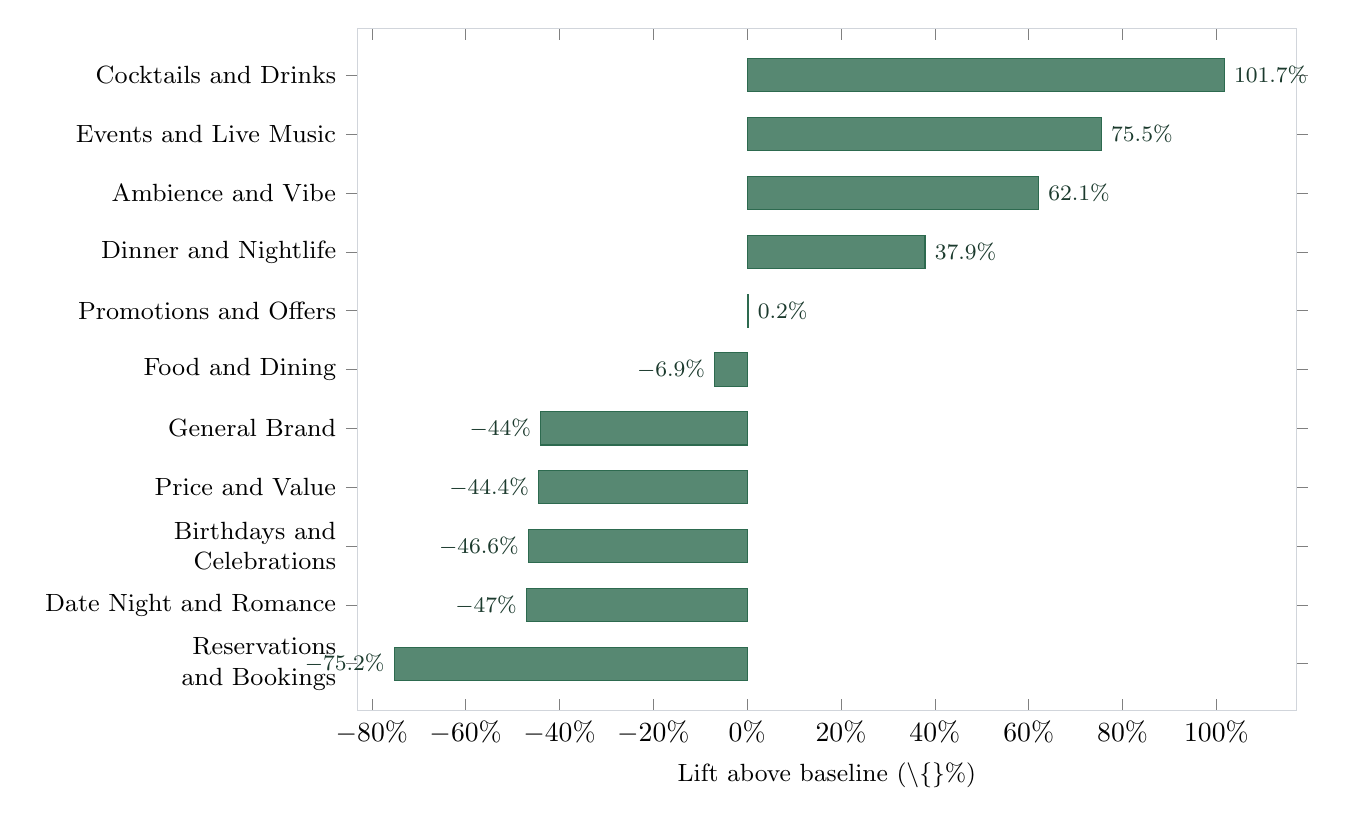
\begin{tikzpicture}
\begin{axis}[
  xbar, xmin=-83, xmax=117,
  width=13.5cm, height=10.25cm, bar width=12pt,
  xlabel={\small Lift above baseline (\textbackslash\{\}\%)},
  symbolic y coords={Reservations and Bookings,Date Night and Romance,Birthdays and Celebrations,Price and Value,General Brand,Food and Dining,Promotions and Offers,Dinner and Nightlife,Ambience and Vibe,Events and Live Music,Cocktails and Drinks}, ytick=data,
  y tick label style={font=\small, align=right, text width=3.8cm},
  scaled x ticks=false,
  xticklabel={\pgfmathprintnumber[fixed,precision=0]{\tick}\%},
  nodes near coords={\pgfmathprintnumber[fixed,precision=1]{\pgfplotspointmeta}\%},
  nodes near coords align={horizontal},
  every node near coord/.style={font=\footnotesize, color=tggreen},
  enlarge y limits=0.08, axis line style={draw=tgrule},
]
\addplot[fill=tgmid!80, draw=tgmid] coordinates {(-75.2,Reservations and Bookings)(-47,Date Night and Romance)(-46.6,Birthdays and Celebrations)(-44.4,Price and Value)(-44,General Brand)(-6.9,Food and Dining)(0.2,Promotions and Offers)(37.9,Dinner and Nightlife)(62.1,Ambience and Vibe)(75.5,Events and Live Music)(101.7,Cocktails and Drinks)};
\end{axis}
\end{tikzpicture}
\end{figure}

\begin{longtable}{@{}L{4cm} R{1.2cm} R{2cm} R{2cm} L{3.5cm}@{}}
\caption{Pillar lift versus baseline with bootstrap 95\textbackslash\{\}\% CI} \\
\toprule
\textbf{Pillar} & \textbf{N} & \textbf{Avg Score} & \textbf{Lift} & \textbf{95\% CI} \\
\midrule
\endfirsthead
\multicolumn{5}{c}{\tablename\ \thetable{} --- continued} \\
\toprule
\textbf{Pillar} & \textbf{N} & \textbf{Avg Score} & \textbf{Lift} & \textbf{95\% CI} \\
\midrule
\endhead
\bottomrule
\endfoot
\bottomrule
\endlastfoot
Cocktails and Drinks & 11 & 289.59 & 101.7\% & 56.86 to 532.39 \\
Events and Live Music & 8 & 251.93 & 75.5\% & 66.95 to 555.72 \\
Ambience and Vibe & 15 & 232.75 & 62.1\% & 108.68 to 388.09 \\
Dinner and Nightlife & 17 & 197.94 & 37.9\% & 54.72 to 393.07 \\
Promotions and Offers & 2 & 143.81 & 0.2\% & 143.81 to 143.81 \\
Food and Dining & 111 & 133.73 & -6.9\% & 82.43 to 188.53 \\
General Brand & 33 & 80.36 & -44\% & 42.65 to 128.02 \\
Price and Value & 2 & 79.84 & -44.4\% & 79.84 to 79.84 \\
Birthdays and Celebrations & 6 & 76.73 & -46.6\% & 43.99 to 109.47 \\
Date Night and Romance & 12 & 76.07 & -47\% & 39.98 to 120.85 \\
Reservations and Bookings & 2 & 35.54 & -75.2\% & 35.54 to 35.54 \\
\end{longtable}

\chapter{Monte Carlo Simulations}
\begin{note}
\textbf{What these simulations are, and are not.} They are \textbf{scenario projections}, not forecasts. Each re-samples from historical pillar engagement under a posting plan and assumes (i) independence, (ii) stationarity, (iii) no saturation, and (iv) inherits small-sample noise. The strategy \textquotedblleft uplift\textquotedblright{} figures are the mechanical consequence of allocating more posts to historically strong categories; the value is the uncertainty band (P5--P95), not point precision.
\end{note}

\section{MC1: Content Strategy Comparison (12 Weeks)}
\begin{table}[htbp]
\centering
\caption{MC1 results: 12-week engagement score by strategy}
\begin{tabular}{@{}L{3cm} R{1.8cm} R{2cm} R{2cm} R{2cm} R{2cm}@{}}
\toprule
\textbf{Strategy} & \textbf{Posts} & \textbf{Mean} & \textbf{P5} & \textbf{P95} & \textbf{Uplift} \\
\midrule
current mix & 58 & 6,773 & 3,696 & 10,378 & --- \\
optimised & 60 & 8,836 & 5,360 & 12,787 & +30.5\% \\
heavy reels & 66 & 12,004 & 7,877 & 16,451 & +77.2\% \\
\bottomrule
\end{tabular}
\end{table}

\section{MC2: Engagement Forecast}
\begin{table}[htbp]
\centering
\caption{MC2: engagement forecast at three horizons}
\begin{tabular}{@{}R{2.5cm} R{2.5cm} R{3cm} R{2.5cm} R{2.5cm} R{1.5cm}@{}}
\toprule
\textbf{Horizon (days)} & \textbf{Exp. Posts} & \textbf{Forecast Mean} & \textbf{P10} & \textbf{P90} & \textbf{CV} \\
\midrule
30 & 16 & 2,087 & 823 & 3,630 & 0.54 \\
60 & 33 & 4,165 & 2,201 & 6,368 & 0.39 \\
90 & 50 & 6,257 & 3,772 & 8,936 & 0.33 \\
\bottomrule
\end{tabular}
\end{table}

\section{MC3: Booking Conversion Pipeline}
\begin{table}[htbp]
\centering
\caption{MC3: monthly booking pipeline under three conversion scenarios}
\begin{tabular}{@{}L{2.5cm} R{1.8cm} R{2cm} R{1.6cm} R{1.6cm} R{1.8cm} R{1.8cm}@{}}
\toprule
\textbf{Scenario} & \textbf{Contact \%} & \textbf{Booking \%} & \textbf{P50} & \textbf{P90} & \textbf{P(0)} & \textbf{P(3+ bookings)} \\
\midrule
pessimistic & 5 & 20 & 0 & 0 & 100\% & 0\% \\
central & 12 & 30 & 0 & 0 & 100\% & 0\% \\
optimistic & 20 & 45 & 0 & 0 & 100\% & 0\% \\
\bottomrule
\end{tabular}
\end{table}
\begin{callout}
\textbf{Principal finding from MC3.} At current comment volumes the Instagram comment channel alone cannot reliably drive booking conversions regardless of conversion rate. The binding constraint is comment volume, not the funnel. Increasing reach-oriented content (MC1) raises the top of the funnel; replying immediately to commercial comments is the cheapest operational lever.
\end{callout}

\section{MC4: Optimal Pillar Mix (Top 10 Allocations)}
\begin{longtable}{@{}L{9cm} R{2.2cm} R{1.8cm} R{1.8cm}@{}}
\caption{MC4: top pillar allocations by expected mean engagement} \\
\toprule
\textbf{Allocation} & \textbf{Mean} & \textbf{P25} & \textbf{P75} \\
\midrule
\endfirsthead
\multicolumn{4}{c}{\tablename\ \thetable{} --- continued} \\
\toprule
\textbf{Allocation} & \textbf{Mean} & \textbf{P25} & \textbf{P75} \\
\midrule
\endhead
\bottomrule
\endfoot
\bottomrule
\endlastfoot
events/live music/DJ:2.17 | cocktails/drinks:0.98 | dinner/nightlife:0.88 | food:0.49 | date night/romance:0.26 | ambience/decor/vibe:0.22 & 10,474 & 8,880 & 12,035 \\
events/live music/DJ:2.21 | cocktails/drinks:0.3 | dinner/nightlife:0.28 | food:0.65 | date night/romance:1.25 | ambience/decor/vibe:0.31 & 9,860 & 8,412 & 11,204 \\
events/live music/DJ:1.99 | cocktails/drinks:0.8 | food:1.51 | date night/romance:0.45 | ambience/decor/vibe:0.21 & 9,774 & 8,154 & 11,245 \\
events/live music/DJ:1.51 | cocktails/drinks:1.87 | dinner/nightlife:0.19 | food:0.17 | date night/romance:1.2 & 9,568 & 7,959 & 10,999 \\
events/live music/DJ:2.1 | cocktails/drinks:0.51 | dinner/nightlife:0.1 | food:1.16 | date night/romance:0.11 | ambience/decor/vibe:1.02 & 9,529 & 8,034 & 10,953 \\
events/live music/DJ:2.13 | cocktails/drinks:0.18 | dinner/nightlife:0.12 | food:0.65 | date night/romance:1.8 | ambience/decor/vibe:0.12 & 9,523 & 8,056 & 10,873 \\
events/live music/DJ:1.55 | cocktails/drinks:1.8 | dinner/nightlife:0.59 | food:0.29 | date night/romance:0.56 | ambience/decor/vibe:0.21 & 9,494 & 7,871 & 10,987 \\
events/live music/DJ:1.7 | cocktails/drinks:0.84 | food:1.77 | date night/romance:0.54 & 9,361 & 7,748 & 10,769 \\
events/live music/DJ:1.45 | cocktails/drinks:1.48 | dinner/nightlife:0.39 | food:0.14 | date night/romance:1.48 & 9,340 & 7,936 & 10,691 \\
events/live music/DJ:1.5 | cocktails/drinks:0.84 | dinner/nightlife:1.55 | food:0.44 | date night/romance:0.63 & 9,322 & 7,679 & 10,928 \\
\end{longtable}

\section{MC5: Risk Analysis}
\begin{longtable}{@{}L{3.2cm} R{2.5cm} R{3cm} R{3cm}@{}}
\caption{MC5: probability of achieving 12-week targets} \\
\toprule
\textbf{Strategy} & \textbf{Target} & \textbf{P(achieve)} & \textbf{Expected Mean} \\
\midrule
\endfirsthead
\multicolumn{4}{c}{\tablename\ \thetable{} --- continued} \\
\toprule
\textbf{Strategy} & \textbf{Target} & \textbf{P(achieve)} & \textbf{Expected Mean} \\
\midrule
\endhead
\bottomrule
\endfoot
\bottomrule
\endlastfoot
current mix & 5,000 & 80\% & 6,771 \\
current mix & 10,000 & 6.9\% & 6,771 \\
current mix & 15,000 & 0\% & 6,771 \\
current mix & 20,000 & 0\% & 6,771 \\
current mix & 30,000 & 0\% & 6,771 \\
current mix & 50,000 & 0\% & 6,771 \\
optimised & 5,000 & 96.6\% & 8,922 \\
optimised & 10,000 & 30.3\% & 8,922 \\
optimised & 15,000 & 0.9\% & 8,922 \\
optimised & 20,000 & 0\% & 8,922 \\
optimised & 30,000 & 0\% & 8,922 \\
optimised & 50,000 & 0\% & 8,922 \\
heavy reels & 5,000 & 99.9\% & 12,043 \\
heavy reels & 10,000 & 78.2\% & 12,043 \\
heavy reels & 15,000 & 12.9\% & 12,043 \\
heavy reels & 20,000 & 0.3\% & 12,043 \\
heavy reels & 30,000 & 0\% & 12,043 \\
heavy reels & 50,000 & 0\% & 12,043 \\
\end{longtable}

\chapter{Limitations and Ethics}
\section{Statistical Scope and Validity}
This study is \textbf{exploratory and hypothesis-generating}, not confirmatory, and is fully reproducible (fixed seed, committed data, deterministic pipeline). Bounds on interpretation:
\begin{enumerate}[leftmargin=*]
\item \textbf{Composite-metric circularity.} The engagement score embeds a views term available to video but not to many image posts; composite-score reels-versus-posts comparisons overstate the advantage, so likes-and-comments comparisons are reported alongside.
\item \textbf{Small samples.} Several pillars and the deduplicated reel set rest on few posts; confidence intervals are wide and rankings are indicative.
\item \textbf{Observational, not causal.} Day, pillar, and format are correlated with each other and with campaign timing; no causal claim is made.
\item \textbf{Scenarios, not forecasts.} Monte Carlo projections assume independence, stationarity, and no saturation.
\item \textbf{Selection effects.} Comments are drawn from high-engagement posts; mentions are a non-random sample.
\end{enumerate}
Used to prioritise content experiments and size uncertainty, the analysis is sound; used as proof of fixed effects, it would overreach.

\section{Data and Ethics}
This report is based on public Instagram data collected via the Apify Instagram Scraper and analysed locally. No private account access or private user data was used. Individual commenters are not identified. For business decisions, combine with Treehouse Ghana's native Instagram Insights, reservation data, and campaign context.

%% SIGN-OFF
\clearpage\thispagestyle{empty}\pagecolor{tggreen}\color{white}\vspace*{5cm}
\begin{center}
{\color{tggold}\rule{8cm}{0.6pt}}\\[28pt]
{\Large\bfseries Prepared by}\\[12pt]
{\fontsize{28}{34}\selectfont\bfseries Bernard Ashiley}\\[14pt]
{\large Odwira and Whitehall}\\[28pt]
{\color{tggold}\rule{8cm}{0.6pt}}\\[22pt]
{\normalsize 2026-05-31}\\[10pt]
{\small\color{white!70!tggreen}All rights reserved. This document is confidential and intended solely\\for the use of Treehouse Ghana and authorised recipients.}
\end{center}
\end{document}
